\documentclass[a4paper,12pt,normaltoc,capchap]{estilos/abnt}
\usepackage{estilos/abnt-UEPG}
\usepackage[top=3cm,bottom=2cm,left=3cm,right=2cm]{geometry}
\usepackage[utf8]{inputenc}
\usepackage[brazil]{babel}
\usepackage[T1]{fontenc}
%\usepackage{hyperref}
\usepackage{amssymb}
\usepackage{amsmath}
\usepackage{paralist}
\usepackage{graphicx}
\usepackage{subfigure}
\usepackage{setspace}
\usepackage{fancyhdr}
\usepackage{lscape}
\usepackage{longtable}
\usepackage{fancyvrb}
\usepackage[alf,abnt-etal-text=it,bibjustif]{estilos/abntcite}
\usepackage{listings}
%\usepackage{fancychap}
\usepackage{makecell}
\usepackage{multirow}
\usepackage{nomencl}
\usepackage{tipa}
\usepackage{array,multirow,graphicx}
\usepackage[table,xcdraw]{xcolor}
\usepackage{pdfpages}
\usepackage{times}
\usepackage{titletoc}
\usepackage{tocbasic}
\usepackage{tabularx}
\usepackage{pifont} 
\renewcommand{\lstlistingname}{Código} % definição visual dos códigos fonte

%%%%%%%% lista de quadros
\usepackage{trivfloat}
\trivfloat{quadro}
\floatstyle{plaintop} % Forçar posição da legenda para o topo
\restylefloat{quadro} % Forçar posição da legenda para o topo
\addto\captionsbrazil{%
\renewcommand{\listquadroname}{Lista de Quadros}}

\renewcommand{\nomname}{Lista de Siglas}
\makeatletter   
\DeclareTOCStyleEntry[
  entrynumberformat=\entrynumberwithprefix{\figurename},
  dynnumwidth,
  numsep=1em
]{tocline}{figure}
\newcommand\entrynumberwithprefix[2]{\hspace{-0.70cm}#1\enspace#2 \hspace{0.22cm} --\hfill }
\renewcommand{\nomname}{Lista de Siglas}

\titlecontents{table}
  [5.5em]
  {}
  {\contentslabel[Tabela~\thecontentslabel~ \hspace{0.1cm} -- \hspace{0.15cm}]{5.5em}}
  {0em}
  {\titlerule*[1pc]{.}\contentspage}

\makeatother


\lstset{language=Java, basicstyle=\footnotesize, numbers=left, frame=tb, breaklines=true, basicstyle=\footnotesize}

%------------------------------------------------------------------------------
% Dicionário de hifenização em português
%------------------------------------------------------------------------------

\hyphenation{pro-ces-sa-men-to}
\hyphenation{a-pre-sen-ta-da}
\hyphenation{pro-gra-ma}
%------------------------------------------------------------------------------
% Configurações da dissertação
%------------------------------------------------------------------------------


\instituicao{UNIVERSIDADE ESTADUAL DE PONTA GROSSA\\
PRÓ-REITORIA DE PESQUISA E PÓS-GRADUAÇÃO\\
PROGRAMA DE PÓS-GRADUAÇÃO EM \\COMPUTAÇÃO APLICADA\\ }

\autor{NOME COMPLETO DO DISCENTE}

\titulo{TITULO DA DISSERTAÇÃO ESCRITO EM LETRA MAIÚSCULA}

\comentario{Projeto de dissertação apresentado para obtenção do título de Mestre em Computação Aplicada na Universidade Estadual de Ponta Grossa, Área de concentração: Escreva a área aqui \\ \\ Orientador: Prof. Dr. Nome do Orientador}

\local{Ponta Grossa}

\data{2020}

%------------------------------------------------------------------------------
% Início do documento 
%------------------------------------------------------------------------------

\begin{document}

\capa

\folhaderosto
%\include{escrita/agradecimentos2} 
%\includepdf[pages=-]{pdfs/Ficha_catalogr_fica.pdf}
%\includepdf[pages=-]{pdfs/ata-aprovacao.pdf}
%\include{escrita/dedicatoria}
%\include{escrita/agradecimentos}
%\include{escrita/resumo}
%\include{escrita/abstract}


\listadefiguras
\listadetabelas

%Para siglas utilizar: listadesiglas ou (makenomenclature e printnomenclature)
\listadesiglas
% \makenomenclature
% \printnomenclature

%\listofquadros
\sumario

\pagestyle{headings}

\lhead{\centering \nouppercase{\rightmark}}
\rhead{\centering \nouppercase{\leftmark}}
\pagestyle{fancy}
\fancyfoot{}
\renewcommand{\chaptermark}[1]{\markboth{\thechapter. \ #1}{}}
\fancyhead[RO, L]{ \thepage}
\fancypagestyle{plain}{
	\fancyhf{}
	\fancyfoot{}
	\renewcommand{\headrulewidth}{0.4pt}
	\renewcommand{\footrulewidth}{0.4pt}
}
\pagestyle{fancy}
\pagenumbering{arabic}
\setcounter{page}{6}

%%%%%%%%%%%%%%%%%%%%%%%%%%%%%%%%%%%%%%%
%             CAPITULOS

%\include{escrita/identificacao}
\chapter{INTRODUÇÃO}

Este é um exemplo de como citar autores
\cite{gibas2001developing}. A Figura \ref{fig:exemplo} é um exemplo que está nas normas da \nomenclature{ABNT}{Associação Brasileira de Normas Técnicas} ABNT.


\begin{figure}[!ht]
\caption{Exemplo de figura nas normas ABNT (BICEN-UEPG).}
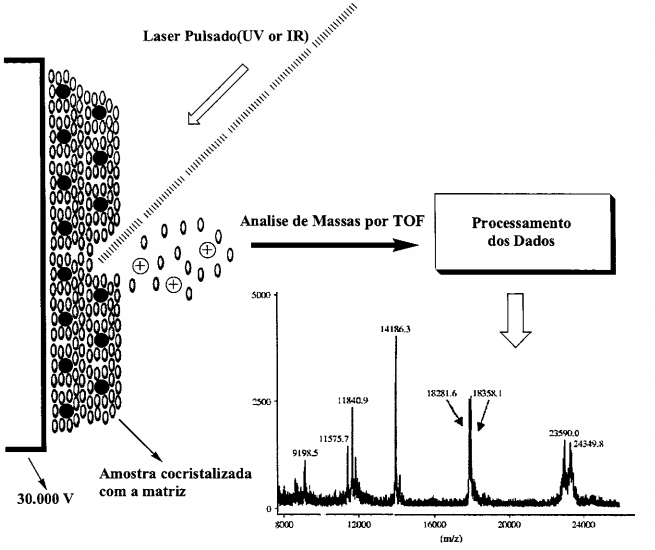
\includegraphics[width=1\textwidth]{imagens/figura1.PNG}
\text{\footnotesize Fonte: \citeonline{gibas2001developing}.}
\label{fig:exemplo}
\end{figure}
%\include{escrita/bjetivo}
\chapter{REVISÃO LITERATURA}

A Bioinformática, também conhecida como Biologia Computacional, consiste na aplicação da informática para resolver problemas biológicos \cite{gibas2001developing}.

\section{EXEMPLO DE SEÇÃO}

A seguir, temos um exemplo de tabela

\begin{table}[!ht]
\caption{Exemplo de Tabela}
\label{ex_tabela}
\begin{tabularx}{\linewidth}{l c X c}
\hline
\multicolumn{1}{l}{\textbf{Experimento}} &
\multicolumn{1}{c}{\textbf{Protocolo}} &
\multicolumn{1}{l}{\textbf{Métrica}} &
\multicolumn{1}{c}{\textbf{Equação}} \\ \hline

Exemplo 1 & 1 & Acurácia Média & 1\\
\hline
Exemplo 2 & 1 & Acurácia Balanceada & 2 \\
\hline
Exemplo 3 & 1 & Média Geométrica & 3 \\
\hline
Exemplo 4 & 2 & \emph{Overfitting} (AM) & 1 e 4 \\
\hline
Exemplo 5 & 2 & \emph{Overfitting} (AB) & 2 e 4 \\
\hline
Exemplo 6 & 3 & Ranqueamento \emph{Relief} & 5 \\ 
\hline
Exemplo 7 & 1 & \emph{AM, AB, OVAM e OVAB} & 1,2 e 4\\ 
\hline
\text{\footnotesize Fonte: O autor.}
\end{tabularx}
\end{table}

\subsection{Exemplo de Subseção}



%\include{escrita/metodologia}
%\include{escrita/resultados}
%\include{escrita/discussao}
%\include{escrita/conclusoes}
%\include{escrita/cronograma}
%\include{escrita/publicacao}

%%%%%%%%%%%%%%%%%%%%%%%%%%%%%%%%%%%%%%%

\bibliographystyle{estilos/abnt-alf}
\bibliography{base}

%\include{Apendice}
%\include{anexo}

\end{document}

%%%%%%%%%%%%%%% 
%%%%%%%%%%%%%%% Fim do documento  
%%%%%%%%%%%%%%%